\section*{Voorbeschouwing}
%\chapterquote{Een computer verdient het om intelligent te worden genoemd, indien hij een mens ervan kan overtuigen, dat hij tegen een mens praat.}{Alan Turing, Brits informaticus (1912-1954)}
\chapterquote{De vraag of computers kunnen denken is net als de vraag of duikboten kunnen zwemmen.}{Edsger Dijkstra, Nederlands informaticus (1930-2002)}%Vragen of computers kunnen denken, is vragen of duikboten kunnen zwemmen.
Artifici\"ele Intelligentie is een gebied binnen de Informatica die vele banden heeft met talloze wetenschappelijke domeinen (bijvoorbeeld Psychologie). De bedoeling van dit domein is het generen van effecten, die door mensen als intelligent worden beschouwd. Dit wil daarom nog niet zeggen dat de structuren die gebouwd worden dit ook effectief zijn (Wat is \"uberhaupt intelligent? De hersenen zijn uiteindelijk ook slechts een machine). Meestal worden deze effecten gegenereerd door een combinatie van enerzijds brute rekenkracht die het niveau van het brein ver overstijgt. Anderzijds door het toepassen van algoritmen die meestal snel naar een oplossing kunnen convergeren.
\paragraph{}
Deze cursus behandelt enkele algemene gebieden in de Artifici\"ele Intelligentie. Daarnaast biedt het ook een korte inleiding op verschillende gebieden die later in andere cursussen verder uitgebreid worden (bijvoorbeeld Machine Learning en Genetische Algoritmen). Deze gebieden zijn:
\begin{itemize}
 \item State-Spaces
 \item Zoekmethodes
 \item Concept Learning (Machine Learning)
 \item Constraint Processing
 \item Game Playing
 \item Automatische Redeneersystemen
 \item Metaheuristieken
\end{itemize}
Uiteraard staan deze gebieden niet los van elkaar. Afhankelijkheden van deze verschillende gebieden worden weergegeven op figuur \ref{fig:partsAndDependenciesOfCourse}. Het is aangewezen om eerst de afhankelijkheden van een bepaald deel te studeren alvorens het deel zelf. De cursus is dan ook zo opgebouwd, dat de afhankelijkheden ondersteund worden. Per hoofdstuk zijn er \'e\'en of meer leidende voorbeelden die gedurende dit hoofdstuk uitgewerkt worden. Alle concepten in het hoofdstuk worden dan op deze voorbeelden toegepast.
\begin{figure}[H]
\centering
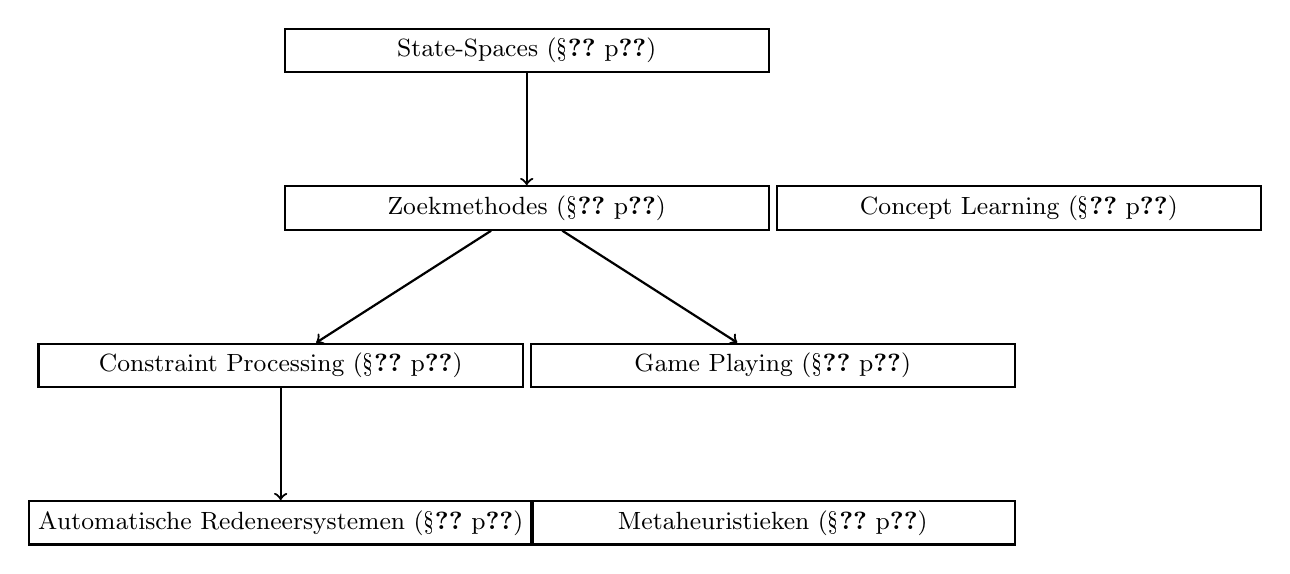
\begin{tikzpicture}[topict/.style={shape=rectangle,draw=black,thick,minimum width=6.15 cm},influences/.style={thick,->}]
\node[topict] (S) at (0,0) {\small State-Spaces (\S\ref{s:stateSpaces} p\pageref{s:stateSpaces})};
\node[topict] (Z) at (0,-2) {\small Zoekmethodes (\S\ref{s:searchMethods} p\pageref{s:searchMethods})};
\node[topict] (CL) at (6.25,-2) {\small Concept Learning (\S\ref{s:conceptLearning} p\pageref{s:conceptLearning})};
\node[topict] (CP) at (-3.125,-4) {\small Constraint Processing (\S\ref{s:constraintProcessing} p\pageref{s:constraintProcessing})};
\node[topict] (G) at (3.125,-4) {\small Game Playing (\S\ref{s:gamePlaying} p\pageref{s:gamePlaying})};
\node[topict] (A) at (-3.125,-6) {\small Automatische Redeneersystemen (\S\ref{s:automaticReasoning} p\pageref{s:automaticReasoning})};
\node[topict] (M) at (3.125,-6) {\small Metaheuristieken (\S\ref{s:metaheuristics} p\pageref{s:metaheuristics})};
\draw[influences] (S) -- (Z);
\draw[influences] (Z) -- (CP);
\draw[influences] (Z) -- (G);
\draw[influences] (CP) -- (A);
\end{tikzpicture}
\caption{Indeling en afhankelijkheden van deze cursus}
\label{fig:partsAndDependenciesOfCourse}
\end{figure}